\chapter{Конструкторский раздел}
\section{Схемы алгоритмов Левенштейна}
Ниже представлены следующие схемы алгоритмов:
\begin{itemize}
	\item рис. \ref{png:1} - схема алгоритма сортировки пузырьком;
	\item рис. \ref{png:2} - схема алгоритма сортировки простыми вставками;
	\item рис. \ref{png:3} - схема алгоритма сортировки методом Шелла.
\end{itemize}

\begin{figure}[pht!]
	\centering{
		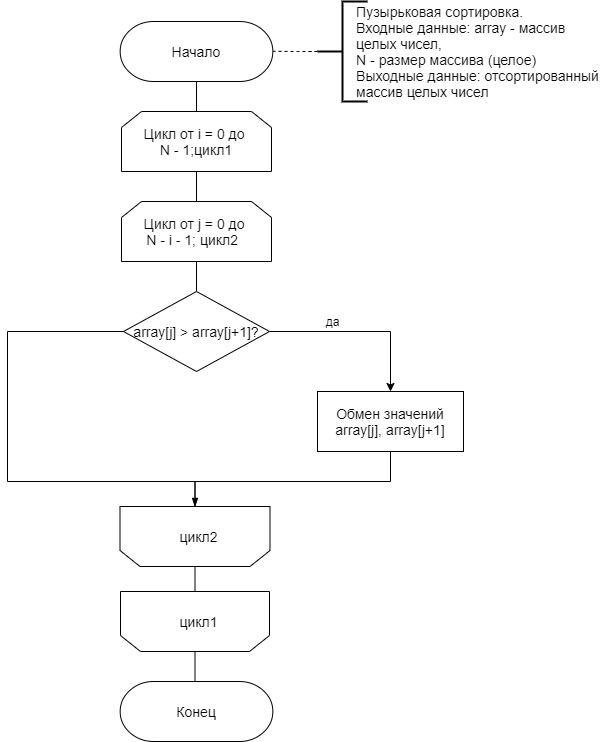
\includegraphics[width=14.6cm]{../../../../../../../msys64/home/Лев/bmstu_sem_5_aa/lab_03/report/diagrams/bubble}
		\caption{Ссхема алгоритма итеративного Левенштейна с использованием двух строк.}
		\label{png:1}}
\end{figure} 

\begin{figure}[pht!]
	\centering{
		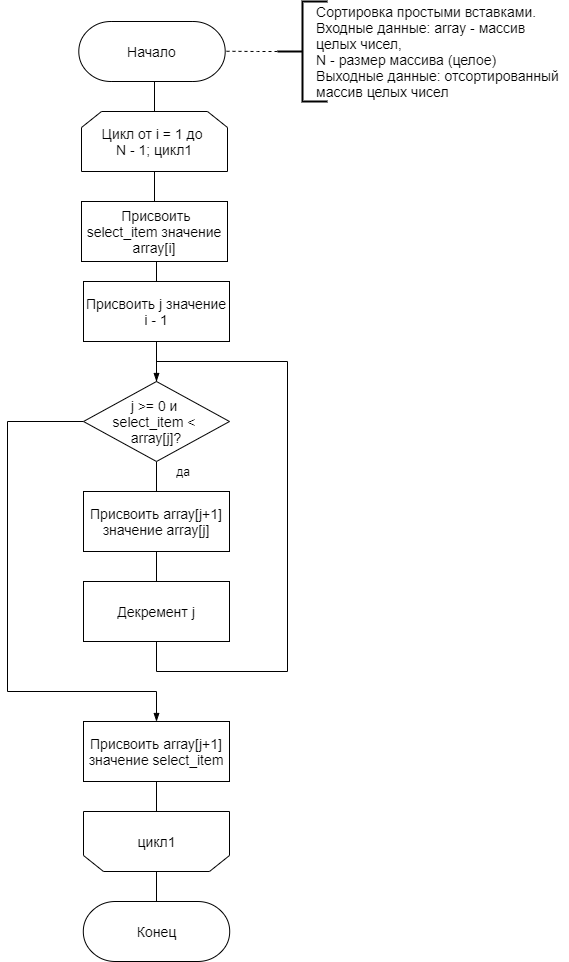
\includegraphics[width=14.6cm]{../../../../../../../msys64/home/Лев/bmstu_sem_5_aa/lab_03/report/diagrams/insert}
		\caption{Схема алгоритма рекурсивного Левенштейна без кэша.}
		\label{png:2}}
\end{figure} 

\begin{figure}[pht!]
	\centering{
		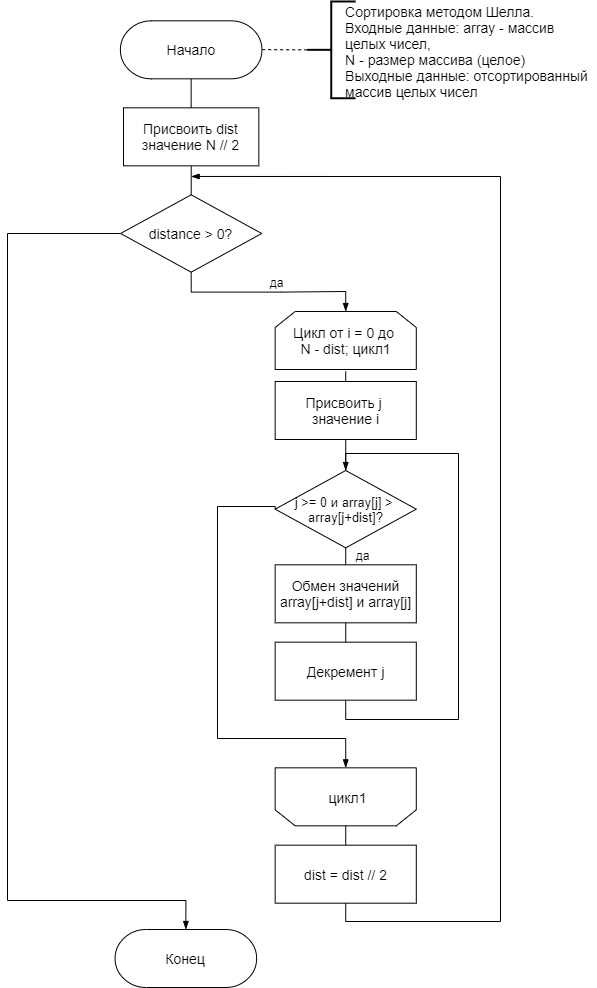
\includegraphics[width=14.6cm]{../../../../../../../msys64/home/Лев/bmstu_sem_5_aa/lab_03/report/diagrams/shell}
		\caption{Cхема алгоритма рекурсивного Левенштейна с использованием матрицы.}
		\label{png:3}}
\end{figure}

\section{Модель оценки трудоемкости алгоритмов}
Введем модель оценки трудоемкости.

\begin{enumerate}
	\item Трудоемкость базовых операций.
	Пусть трудоемкость операций *, /, \, //, \%, *=, /= равна 2. 
	
	Примем трудоемкость следующих операций равной 1:
	
	=, +, -, +=, -=, ==, !=, <, >, <=, >=, |, \&\&,, ||, []  
	\item Трудоемкость цикла.
	Пусть трудоемкость цикла определяется по формуле \ref{eq1}:
	
	\begin{equation}
	\label{eq1} 
	f = f_{init} + f_{comp} + N_{iter} * (f_{in} + f_{inc} + f_{comp})
	\end{equation} 
	где:
	\begin{itemize}
	\item $f_{init}$ - трудоемкость инициализации переменной-счетчика;
	\item $f_{comp}$ - трудоемкость сравнения;
	\item $N_{iter}$ - номер выполняемой итерации;
	\item $f_{in}$ - трудоемкость команд из тела цикла;
	\item $f_{inc}$ -трудоемкость инкремента;
	\item $f_{comp}$ - трудоемкость сравнения.
	\end{itemize}
	\item Трудоемкость условного оператора. \\
	Пусть трудоемкость самого условного перехода равна 0, но она определяется по формуле \ref{eq2}. 
	\begin{equation}
		\label{eq2}
		f_{if} = f_{comp\_if} + \begin{cases}
								f_{a}\\
								f_{b}\\
								\end{cases}
	\end{equation}

\end{enumerate}
	

\section{Вычисление трудоемкости алгоритмов}
Пусть размер массивов во всех дальнейших вычислениях обозначается как N.
\subsection{Трудоемкость пузырька}
Трудоемкость этого алгоритма сортировки состоит из:

\begin{itemize}
	\item трудоемкость внешнего цикла вычисляется по формуле \ref{eq3};
	\begin{equation}
		\label{eq3} 
		f_{i} = {\underset{=}{1}} + {\underset{<}{1}} + N= 2 + N
	\end{equation}

	\item трудоемкость внутреннего цикла вычисляется по формуле \ref{eq4};
	\begin{equation}
		\label{eq4} 
		f_{j} = {\underset{i++}{2}} + {\underset{=}{1}} + {\underset{<}{1}} + {\underset{-}{1}} +
				\frac{N-1}{2}*({\underset{j++}{2}} + f_{if}) = 6 + \frac{N-1}{2}*(2 + f_{if})
	\end{equation}

	где вычисление худшего/лучшего случая определяется по формуле \ref{eq5}:
	 \begin{equation}
	 	\label{eq5}
	 	f_{if} = {\underset{>}{1}} + {\underset{[\ ]}{2}} + {\underset{+}{1}} +
	 	\begin{cases}
	 		0\\
	 		{\underset{=}{3}} + {\underset{[\ ]}{4}} +{\underset{+}{2}}\\
	 	\end{cases}
 		=
 		\begin{cases}
 			0, \text{  лучший случай}\\
 			9, \text{  худший случай}
 		\end{cases}
	 \end{equation}
 
 	Итоговая трудоемкость рассчитывается по формуле \ref{eq6}:
 	\begin{equation}
 		\label{eq6}
 		f_{sum} = f_{i} * f_{j} \approx O(N^2)
 	\end{equation}
 	
 	Трудоемкость пузырька для лучшего случая \ref{eq7}:
 	\begin{equation}
 		\label{eq7}
 		f_{sum} = 3N^2 + 3N + 2 \approx O(N^2)
 	\end{equation}
 
	 Трудоемкость пузырька для худшего случая \ref{eq8}:
	 \begin{equation}
	 	\label{eq8}
	 	f_{sum} = 7.5N^2 - 1.5N + 2 \approx O(N^2)
	 \end{equation}

\end{itemize}
\subsection{Трудоемкость вставок}
\subsection{Трудоемкость Шелла}


\section*{Вывод}
На основе теоретических данных, полученных в аналатическом разделе, были построены схемы нужных алгоритмов.